Los resultados obtenidos en cada uno de los pasos de este trabajo se detallan
en este capítulo, comenzando por el motor obtenido en la primer iteración de
optimización con el algoritmo genético, luego se presenta el modelo de CAD
generado para la segunda etapa de simulación.

Luego se muestran los resultados de las flujometrías realizadas con la
geometría obtenida, incluyendo las mallas obtenidas para algunos casos
seleccionados y el resultado detallado de algunas de las flujometrías,
finalizando con el mapa de coeficientes de descarga obtenido, tanto para el
puerto de admisión como para el puerto de escape.

Por último se presentan los resultados de la segunda ronda de optimización con
el algoritmo genético, en la que se utilizó el mapa de coeficientes de descarga
obtenido en el paso previo.
%
En esta sección se muestra además el modelo de CAD generado para esta
geometría.

% %%%%%%%%%%%%%%%%%%%%%%%%%%%%%%%%%%%%%%%%%%%%%%%%%%%%%%%%%%%%%%%%%%%%%%%%%%%%%%%
%
% \subsection{Metodología}
%
Se simulará un MRCVC de 3 paletas usando el simulador de motores de combustión
interna ICESym~\parencite{icesym} con el propósito de obtener curvas de
rendimiento volumétrico.
%
Estas serán el principal criterio para evaluar el diseño de los sistemas de
intercambio de gases, que consisten de los puertos y conductos.
%
La geometría se optimizará mediante un algoritmo genético, el cual transforma
los datos de rendimiento volumétrico en un puntaje representativo de cada
motor.


La simulación con ICESym requiere del conocimiento previo de los coeficientes
de descarga de los puertos, en la primer iteración se asume un valor constante
para cada puerto que vale 0.7 y 0.75 para admisión y escape respectivamente.
%
Se utilizará la geometría obtenida en esta primer iteración para crear modelos
en CAD de los puertos de admisión y escape, junto con una porción de la cámara
de combustión para realizar flujometrías virtuales.
%
De este modo se puede obtener los coeficientes de descarga de cada puerto en
distintos grados de apertura.

Con el resultado de las flujometrías se construye un mapa del $C_D$ en función
de la alzada, que representa la posición del puerto y la diferencia de presión
entre el puerto y la cámara de combustión.

Este mapa se introduce en ICESym y se vuelve a realizar el proceso de
optimización con el algoritmo genético.

El Simulador de Motores de Combustión Interna (ICESym) permite la simulación de
motores tanto alternativos como rotativos en general y el MRCVC en particular,
en su código se incluyen modelos de la geometría del motor, la transferencia de
calor y el solape de cámaras.

%%%%%%%%%%%%%%%%%%%%%%%%%%%%%%%%%%%%%%%%%%%%%%%%%%%%%%%%%%%%%%%%%%%%%%%%%%%%%%%


%%%%%%%%%%%%%%%%%%%%%%%%%%%%%%%%%%%%%%%%%%%%%%%%%%%%%%%%%%%%%%%%%%%%%%%%%%%%%%%

\section{CAD}
%
El modelo 3D de los puertos de admisión, escape y los componentes internos del
motor que afectan el flujo y son relevantes a la flujometría se realizaron con
FreeCAD\parencite{freecad} para generar un archivo en formato \emph{.BREP} para cada
posición analizada.
%
Estos archivos son importados al software salome\parencite{salome}, ese permite
generar una malla cerrada que se puede utilizar para OpenFOAM.\@
%
Antes de generar la malla se aplican los nombres de los parches, en los que
luego se toman de referencia para aplicar las reglas para realizar el
refinamiento con snappyHexMesh, aplicar condiciones de contorno, iniciales y
demás.
%
Se genera la malla con el mallador NETGEN 1D-2D-3D y se exporta parche por
parche en formato \emph{ASCII.stl}.

%
El archivo \emph{stl} se utiliza en OpenFOAM para generar la malla con
\emph{snappyHexMesh}.

Dada la cantidad de geometrías posibles y el tiempo que toma el proceso, se
realizaron algunas simplificaciones, las cuales se listan a continuación.

%%%%%%%%%%%%%%%%%%%%%%%%%%%%%%%%%%%%%%%%%%%%%%%%%%%%%%%%%%%%%%%%%%%%%%%%%%%%%%%

% \subsection{Geometría}
%
\begin{enumerate}

    \item La interfaz entre los puertos de admisión y escape con sus respectivos
        conductos de conexión con la atmósfera es de sección circular.
        %
    \item La altura de la ranura se adopta en $2/3$ del alto de la cámara,
        siendo $h_c=\lua{tex.print(myData.hc)}\ mm$.
        %
    \item El eje del puerto se hace perpendicular a una línea que pasa entre el
        centro del motor y el la línea media del puerto.
\end{enumerate}


%%%%%%%%%%%%%%%%%%%%%%%%%%%%%%%%%%%%%%%%%%%%%%%%%%%%%%%%%%%%%%%%%%%%%%%%%%%%%%%

\section{Primer Iteración}
%
La primer optimización se realizó partiendo de una población al azar, con los
coeficientes de descarga constantes de 0.7 y 0.75 para el puerto de admisión y
escape respectivamente.
%
El algoritmo genético se ejecutó durante 100 generaciones con una población de
100 individuos, con la función objetivo definida en la
sección~\ref{capitulo:MARCOTEORICO} con los pesos indicados, operadores y
parámetros correspondientes indicados en la tabla~\ref{tab:config_genetico}.

\begin{table}[h]
  \centering
  \begin{tabular}{cc} \toprule
    Parámetro & Valor \\ \midrule
    RPMS & $(1000, 2000, 3000, 4000, 5000, 6000, 7000, 8000, 9000)$ \\
    Pesos de función objetivo & $(1, 1, 1, 6, 8, 9, 8, 7, 7)$ \\
    Cantidad de ciclos de ICESym & 2 \\
    Diámetro mínimo & 0.05 \\
    Diámetro máximo & 0.1 \\
    Longitud mínima de tubo & 0.5 \\
    Longitud máxima de tubo & 2 \\
    Ángulo mínimo & 0 \\
    Ángulo máximo & 90 \\
    Separación angular máxima & 70 \\
    Tamaño de población & 100 \\
    Tamaño de torneo & 10 \\
    $\mu$ & 0 \\
    $\sigma$ & 1 \\
    $\alpha$ & 0.5 \\
    Probabilidad de cruza & 0.9 \\
    Probabilidad de mutación & 0.5 \\
    Cantidad de generaciones & 20 \\
    Tamaño de \emph{SALÓN DE LA FAMA} & 1 \\ \bottomrule
    \end{tabular}
  \caption{Configuración utilizada.}\label{tab:config_genetico}
\end{table}

Para ICESym se utilizaron dos ciclos de simulación, por considerarse que es
suficientemente preciso para esta primer aproximación.
%
En la figura XX se puede ver que a partir de la segunda iteración se obtienen
buenos resultados, esto se debe a que los datos de partida para la segunda
iteración, son los resultados de la primer iteración.

En la gráfica de evolución se observa  que se obtuvo rápidamente un individuo
con un puntaje relativamente alto en en las primeras iteraciones, el resultado
final tiene una aptitud 1.5 veces la aptitud media de la población, los
parámetros que definen este candidato son los listados en la tabla y se
ilustran en la figura~\ref{fig:pop_ev_1}.
%
Este motor tiene un rendimiento volumétrico máximo de $r_{v} = 0.84$ para 3500
rpm y si bien la función objetivo favorece curvas suaves, se ven dos picos de
rendimiento en la curva, siendo el segundo con $r_{v} = 0.81$ a 8000 rpm.

\begin{center}
  \begin{tabular}{rl}
    \begin{tikzpicture}[baseline, trim axis left]
      \begin{axis}[
        xlabel=Generación,
        ylabel=Puntaje,
    legend pos=south east,
        grid=major,
        ]
        \addplot table [x=Gen,y=Avg]{data/genetico.dat} ;
        \addplot table [x=Gen,y=Max]{data/genetico.dat} ;
        \legend{Máximo, Media}
      \end{axis}
    \end{tikzpicture}
    &
    \begin{tikzpicture}[baseline, trim axis right]
      \begin{axis}[
        xlabel=RPM,
        yticklabel pos=upper,
        ylabel={$rend_{vol}$},
        ylabel near ticks,
        grid=major,
        ]

        \addplot table [x=RPM,y=RendVol]{data/primer_rend_vol.dat} ;

      \end{axis}
    \end{tikzpicture}
    \\
  \end{tabular}
  % \caption{Primer Iteración}
  % \label{fig:primer_op}
\end{center}

\begin{table}
  \centering
  \begin{tabular}{ccc} \toprule
    Parámetro & Valor & Unidad \\ \midrule
    DTA & 97.24 & mm\\
    DTE & 81.15 & mm\\
    LIT & 519.31 & mm\\
    LET & 976.66 & mm\\
    IIA & 1.12 & grado\\
    IFA & 70.15 & grado\\
    EIA & 85.14 & grado\\
    EFA & 11.13 & grado\\ \bottomrule
  \end{tabular}
  \caption{Mejor Candidato.}\label{tab:resultado_primer_it}
\end{table}

En la figura XXX se muestran las curvas de potencia y torque del motor, como es
de esperarse se ve que ambas copian la curva de rendimiento volumétrico, con
una potencia máxima de XXX HP a 1000 rpm y un torque máximo de xxxx N.m. a xxx
rpm.

%%%%%%%%%%%%%%%%%%%%%%%%%%%%%%%%%%%%%%%%%%%%%%%%%%%%%%%%%%%%%%%%%%%%%%%%%%%%%%%

\subsection{Puerto de admisión}

Evaluando las curvas de presión para estas rpm se observa que durante la
apertura del puerto de escape hay una depresión de XXX Pa, para este punto el
coeficiente de descarga se estima en XXX y fluje un XX porciento de la masa
total que ingresa durante el período angular en que se encuentra abierto el
puerto.

El puerto de escape ocupa un período angular de $69^{\circ}$, inciando la
apertura en $1.12^{\circ}$ y cerrando a $70.15^{\circ}$ en relación al giro del
cigüeñal.

Se puede concluir que el puerto de admisión tiene sintonías en XXX, XXX, XXX
rpm, siendo los diferenciales de presión mayores en xxx xxx xxx.

%%%%%%%%%%%%%%%%%%%%%%%%%%%%%%%%%%%%%%%%%%%%%%%%%%%%%%%%%%%%%%%%%%%%%%%%%%%%%%%

\subsection{Puerto de escape}
%
El puerto de escape ocupa un período angular de $69^{\circ}$, inciando la
apertura en $1.12^{\circ}$ y cerrando a $70.15^{\circ}$ en relación al giro del
cigüeñal.

%%%%%%%%%%%%%%%%%%%%%%%%%%%%%%%%%%%%%%%%%%%%%%%%%%%%%%%%%%%%%%%%%%%%%%%%%%%%%%%

\section{Modelo de CAD}
%
Los parámetros geométricos obtenidos se utilizaron para modelar los puertos,
tratando de generar una transición suave entre puerto y cámara de combustión
para favorecer el pasaje de gas.
%
Como se ve en la figura~\ref{fig:motor_cad}, se redondearon las aristas
internas incluyendo las paletas y las puntas del rotor, esto para favorecer el
proceso de mallado requerido en el paso siguiente a este ya que los bordes
agudos son complejos de adaptar a una malla construida con tetraedros, como lo
es la malla resultante de snappyHexMesh que se describió en el apartado xxx del
capítulo xxx.

\begin{figure}
  \centering
    \begin{subfigure}{0.4\textwidth}
        \centering
        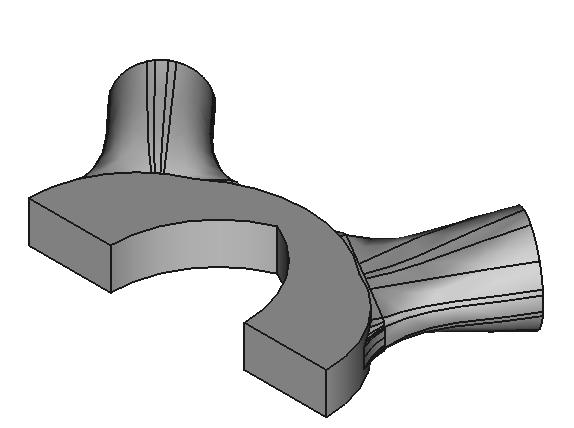
\includegraphics[width=\textwidth]{CAD/motor_cad1.png}
    \end{subfigure}
    \hfill
    \begin{subfigure}{0.4\textwidth}
        \centering
        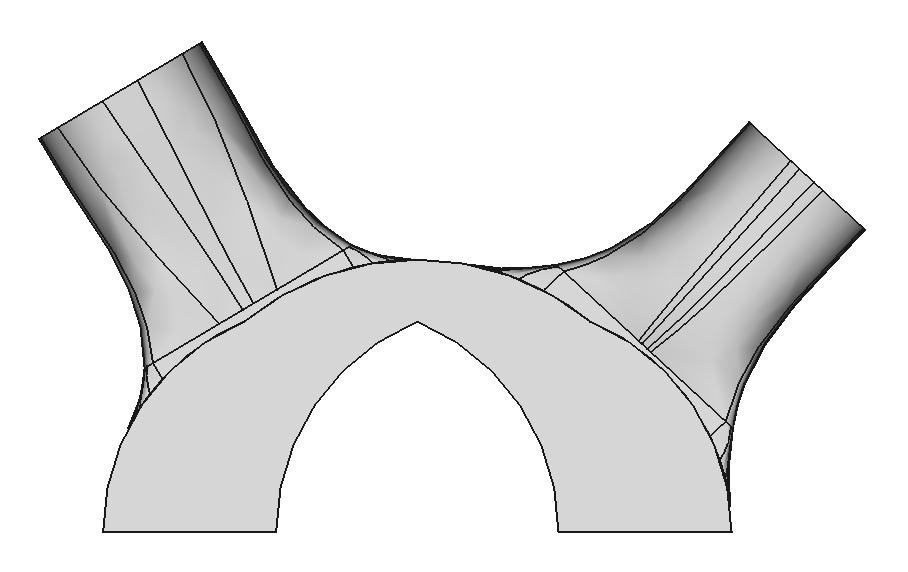
\includegraphics[width=\textwidth]{CAD/motor_cad2.png}
    \end{subfigure}
  \caption{CAD Primer Iteración}\label{fig:motor_cad1}
\end{figure}

La altura del puerto del lado de la cámara de combustión se mantuvo en dos
tercios del a altura de cámara.

\begin{figure}
  \centering
    \begin{subfigure}{0.8\textwidth}
        \centering
        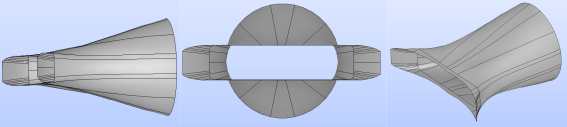
\includegraphics[width=\textwidth]{CAD/vistas_admision.png}
        \caption{Puerto de Admsisión.}
    \end{subfigure}
    \begin{subfigure}{0.8\textwidth}
        \centering
        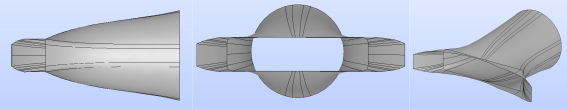
\includegraphics[width=\textwidth]{CAD/vistas_escape.png}
        \caption{Puerto de Escape.}
    \end{subfigure}
  \caption{CAD Primer iteración (vistas fuera de escala).}\label{fig:motor_cad2}
\end{figure}

%%%%%%%%%%%%%%%%%%%%%%%%%%%%%%%%%%%%%%%%%%%%%%%%%%%%%%%%%%%%%%%%%%%%%%%%%%%%%%%
\section{Flujometrías}

De los resultados de la primer otpimización se extrajo una curva de diferencia
de presión vs alzada en diferentes velocidades del motor con el finde de
identificar los puntos de mayor interés para realizar las flujometrías,
tratando de obtener una buena cobertura del rango de funcionamiento de cada
puerto.

% Inicialmente se propusieron un total de XXX flujometŕias, sin embargo algunas
% combinaciones de $\l_{v}, \Delta P$ no se pudieron ejecutar hasta la
% convergencia del flujo másico, por lo que se redujo la cantidad de flujometrías
% final a xxx flujometrías, xxx para el puerto de admisión y xxx para el puerto
% de escape, el par  se detalla en la figura XXX y tabla xxx.

Los pares $(\l_{v}, \Delta P)$ se detallan en la figura XXX, en estos puntos se
flujó el puerto para luego se calcular el coeficiente de descarga, obteniendo
la base para generar el mapa de $C_D$ que se utilizará en el próximo paso de
simulación.

Como se mencionó en el apartado~\ref{capitulo:DESARROLLO}, la modificaión
realizada a ICESym para funcionar con un mapa de $C_{D}$ dependiente de dos
variable, requiere que los datos de entrada estén distribuidos en una grilla
rectangular, motivo por el cual a partir de estos valores se utilizó el método
de interpolación por IDW para generar una dicha grilla de $(l_{v}, \Delta P)$
con $C_{D}$ interpolado de los datos conocidos, como se ve en las
figuras~\ref{fig:mapa_cd_admision} y~\ref{fig:mapa_cd_escape}.

\begin{figure}
    \centering
    \begin{subfigure}{0.4\textwidth}
        \centering
        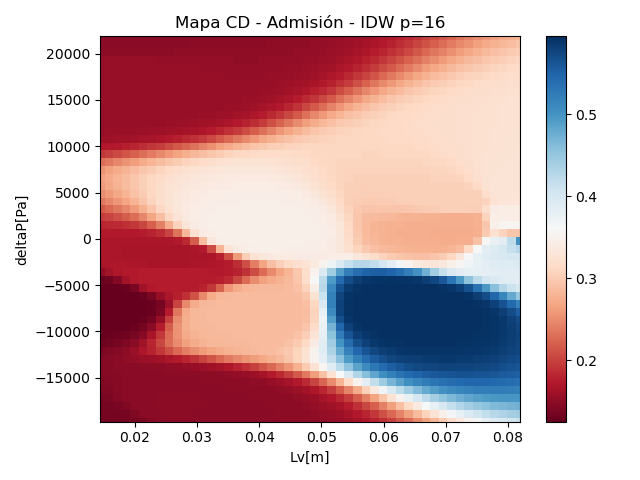
\includegraphics[width=\textwidth]{mapa_cd/idw16_mapa_adm.png}
        \caption{cambiar}
    \end{subfigure}
    \hfill
    \begin{subfigure}{0.4\textwidth}
        \centering
        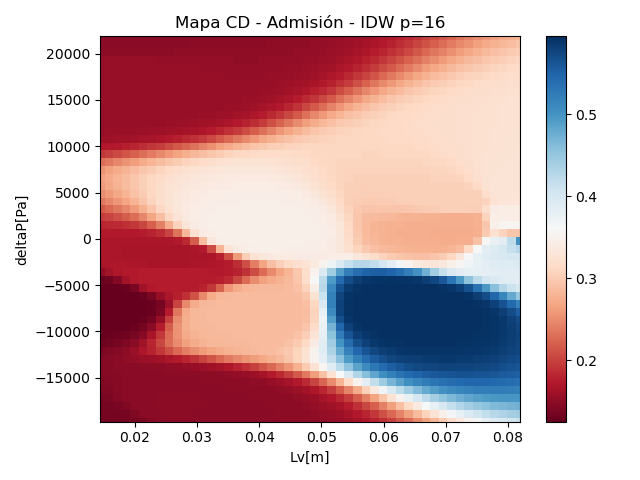
\includegraphics[width=\textwidth]{mapa_cd/idw16_mapa_adm.png}
        \caption{cambiar}
    \end{subfigure}
    \caption{cabmiar}\label{fig:mapa_cd_admision}
\end{figure}

\begin{figure}
    \centering
    \begin{subfigure}{0.4\textwidth}
        \centering
        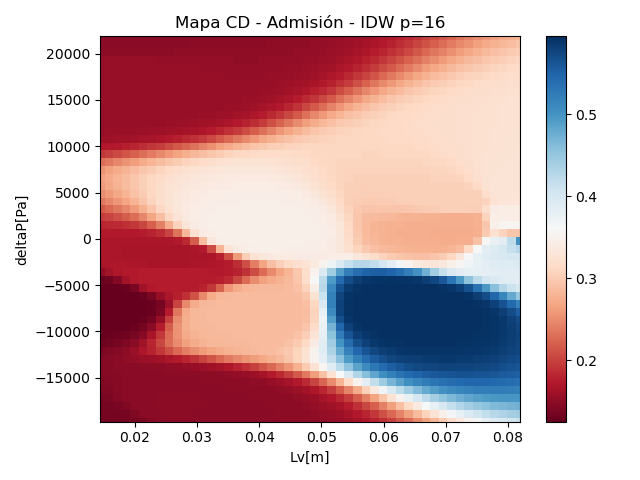
\includegraphics[width=\textwidth]{mapa_cd/idw16_mapa_adm.png}
        \caption{cambiar}
    \end{subfigure}
    \hfill
    \begin{subfigure}{0.4\textwidth}
        \centering
        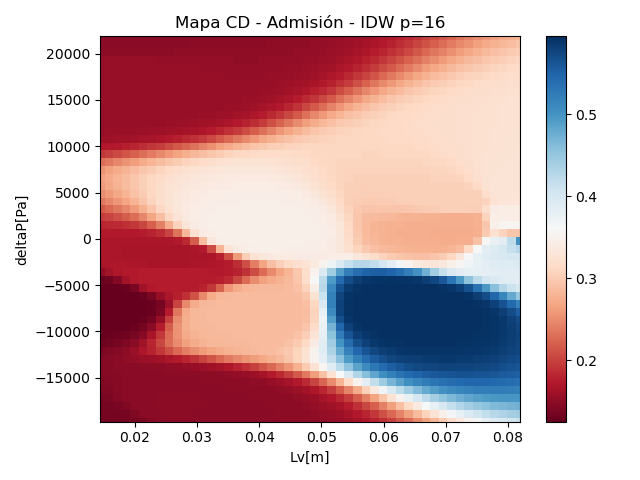
\includegraphics[width=\textwidth]{mapa_cd/idw16_mapa_adm.png}
        \caption{cambiar}
    \end{subfigure}
    \caption{cabmiar}\label{fig:mapa_cd_escape}
\end{figure}

En el mapa del puerto de admisión se observa un máximo para para aperturas del
puerto mayores a 80mm, con $\Delta P$ de entre 1000 Pa a 15000 Pa.
%
El coefiente de descarga máximo es $C_{D}(100mm, 1500Pa) = 0.6$ y corresponde a
la flujometría $N^{\circ} X$, el flujo másico obtenido para este régimen es de
0.02 kg/s, con un a velocidad máxima de xxx m/s en la garganta.
%
El peor valor se es $C_{D}(100mm, 1500Pa) = 0.6$ y corresponde a aperturas
pequeñas del puerto, en la que debido a la reducida sección de pasaje de flujo
se tiene velocidades eleveadas, siendo la máxima de xxx m/s.
%
Para visualizar la diferencia entre uno y otro caso, se representan las líneas
de corriente para ambos casos en la figura
\ref{fig:comparativa_lineas_corriente}.

\begin{figure}
    \centering
    \begin{subfigure}{0.4\textwidth}
        \centering
        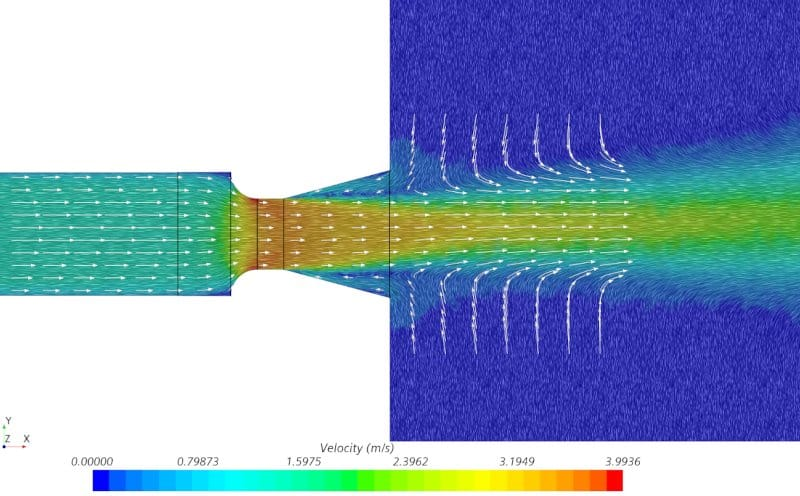
\includegraphics[width=\textwidth]{flujometrias/ejemplo_lineas_corriente.jpg}
        \caption{Valor máximo de $C_{D}$}
    \end{subfigure}
    \hfill
    \begin{subfigure}{0.4\textwidth}
        \centering
        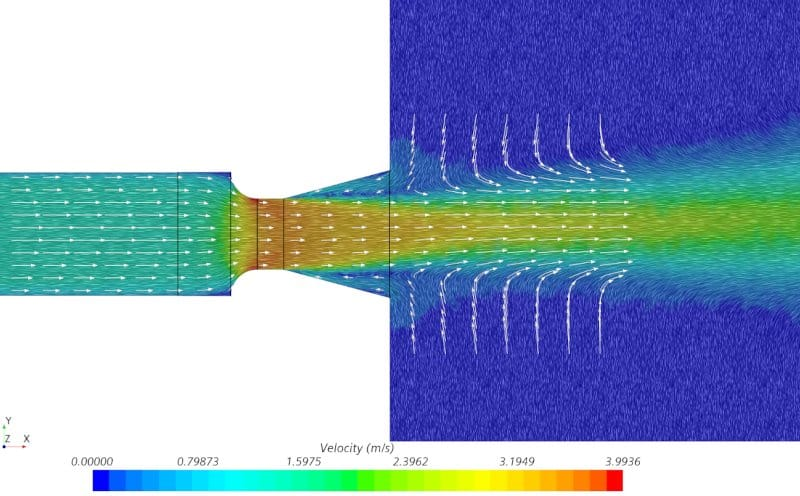
\includegraphics[width=\textwidth]{flujometrias/ejemplo_lineas_corriente.jpg}
        \caption{Valor mínimo de $C_{D}$}
    \end{subfigure}
    \caption{cabmiar}\label{fig:comparativa_lineas_corriente}
\end{figure}

Para el mapa del puerto de escape se observa un máximo para para aperturas del
puerto mayores a 80mm, con $\Delta P$ de entre 1000 Pa a 15000 Pa.
%
El coefiente de descarga máximo es $C_{D}(100mm, 1500Pa) = 0.6$ y corresponde a
la flujometría $N^{\circ} X$, el flujo másico obtenido para este régimen es de
0.02 kg/s, con un a velocidad máxima de 10m/s en la garganta, como se ve en la
figura \ref{fig:admision_10_2000.jpg}.

\begin{figure}
    \centering
    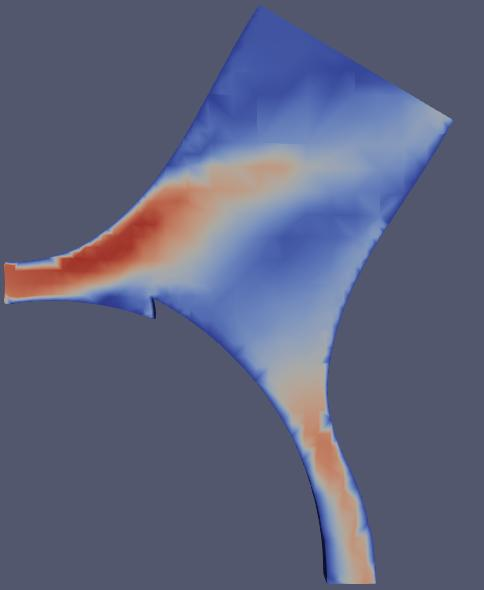
\includegraphics[width=0.7\textwidth]{flujometrias/admision_10_2000.jpg}
    \caption{Puerto de admisión - $10^{\circ}$@2000 RPM}\label{fig:admision_10_2000.jpg}
\end{figure}

El peor valor se es $C_{D}(100mm, 1500Pa) = 0.6$ y corresponde a aperturas
pequeñas del puerto, en la que debido a la reducida sección de pasaje de flujo
se tiene velocidades eleveadas, siendo la máxima de xxx m/s.
%
Para visualizar la diferencia entre uno y otro caso, se representan las líneas
de corriente para ambos casos en la figura \ref{fig:admision_10_2000.jpg}.

\begin{figure}
    \centering
    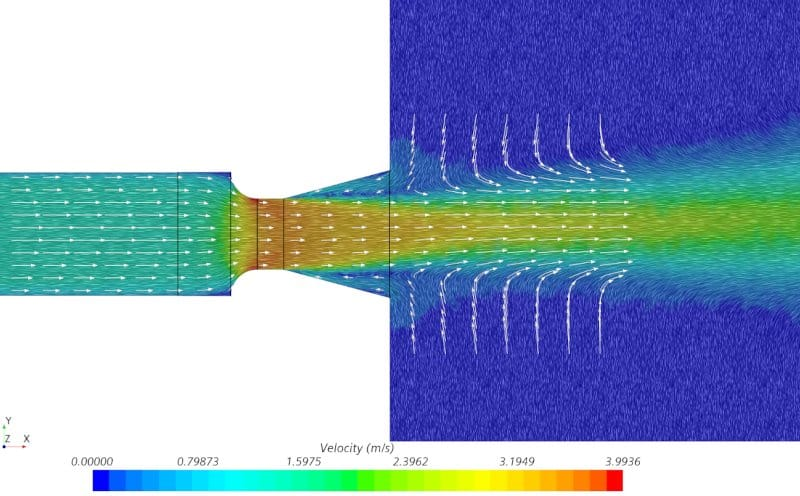
\includegraphics[width=0.7\textwidth]{flujometrias/ejemplo_lineas_corriente.jpg}
    \caption{Puerto de admisión - $10^{\circ}$@2000 RPM}\label{fig:admision_10_2000.jpg}
\end{figure}

En las tablas~\ref{tab:mapa_cd_admision} y~\ref{tab:mapa_cd_escape} se muestran los
resultados de realizar las flujometrías de los puertos de admisión y escape.

\begin{table}
  \centering
    \begin{tabular}{cccc} \toprule
      Caso  & lv        & $\Delta P$    & $C_{D}$   \\ \midrule
      0     & 0.016826  & -100331.39    &  0.213882 \\
      0     & 0.106775  & 5723.72       &  0.489375 \\
      0     & 0.016826  & -263797.72    &  0.011021 \\
      0     & 0.106775  & -3296.18      &  0.803197 \\
      0     & 0.016826  & -652902.78    &  0.011106 \\
      0     & 0.106775  & -9613.29      &  0.815804 \\
      0     & 0.016826  & -513568.73    &  0.011280 \\
      0     & 0.106775  & -3232.97      &  0.813186 \\
      1     & 0.026960  & -116996.12    &  0.375219 \\
      1     & 0.096641  & -3643.9       &  0.878414 \\
      1     & 0.026960  & -237724.11    &  0.018632 \\
      1     & 0.096641  & -6684.11      &  0.867774 \\
      1     &  0.02696  & -496509.46    &  0.111212 \\
      1     &  0.09664  & -18256.20     &  0.805830 \\
      1     & 0.026960  & -237724.11    &  0.022716 \\
      1     & 0.096641  & -6684.11      &  0.862647 \\
      2     & 0.047228  & -49343.47     &  0.541857 \\
      2     & 0.076373  & -5712.86      &  0.918061 \\
      2     & 0.047228  & -109348.67    &  0.487137 \\
      2     & 0.076373  & -17090.38     &  0.914182 \\
      3     & 0.067496  & 13.83         &  0.696967 \\
      3     & 0.071759  & -134.24       &  0.707263 \\
      3     & 0.067496  & -100073.52    &  0.731100 \\
      3     & 0.071759  & -24077.34     &  0.723965 \\
      4     & 0.075750  & -11793.31     &  0.946392 \\
      4     & 0.087764  & -33418.12     &  0.235717 \\
      4     & 0.087764  & -10715.70     &  0.221632 \\
      4     & 0.075750  & -5167.81      &  0.897169 \\
      6     & 0.123601  & -73.94        &  0.878522 \\ \bottomrule
    \end{tabular}
  \caption{Mapa de $C_D$ del puerto de escape} \label{tab:mapa_cd_escape}
\end{table}

\begin{table}
  \centering
  \begin{tabular}{cccc} \toprule
      Caso  & lv        & $\Delta P$    & $C_{D}$   \\ \midrule
      0     & 0.014432  & -6574.97      &  0.206543 \\
      0     & 0.081937  & -87.24        &  0.828822 \\
      0     & 0.014432  & 21856.29      &  0.243975 \\
      0     & 0.081937  & -573.65       &  0.738459 \\
      0     & 0.014432  & -19738.67     &  0.222406 \\
      0     & 0.081937  & 519.60        &  0.487115 \\
      0     & 0.081937  & 1571.95       &  0.587277 \\
      0     & 0.014432  & 18077.97      &  0.256415 \\
      0     & 0.014432  & 2668.61       &  0.247292 \\
      0     & 0.081937  & 0.98          &  0.025970 \\
      2     & 0.062951  & -297.79       &  0.816487 \\
      2     & 0.081937  & 292.92        &  0.466147 \\
      2     & 0.062951  & -7374.88      &  0.980617 \\
      2     & 0.081937  & 4953.85       &  0.541619 \\
      3     & 0.071763  & 4092.13       &  0.501641 \\
      3     & 0.025832  & -3689.81      &  0.289852 \\
      4     & 0.069767  & -789.00       &  0.615690 \\
      4     & 0.069767  & 7869.92       &  0.599348 \\
      4     & 0.005564  & -12539.15     &  0.534555 \\
      4     & 0.005564  & -10091.84     &  0.583979 \\ \bottomrule
    \end{tabular}
  \caption{Mapa de $C_d$ del puerto de Admisión} \label{tab:mapa_cd_admision}
\end{table}


La geometría obtenida luego de realizar la optimización con los mapas de $C_D$
incorporados a la simulación de ICESym se muestra en la figura \ref{fig:geom_nueva}.
%
Se puede ver que la geometría es similar a la inicial, siendo el puerto de
admisión algo menor en cuanto a diámetro que en el caso inicial.

Como es de esperarse, incorporar estos mapa al modelo del motor tiene un efecto
en el comportamiento del mismo, esto se puede observar principalmente en las
curvas de presión del motor.

\subsection{Mapa de $C_D$}
%
Para obtener el mapa se tomaran valores de flujo másico en las combinaciones de
$(\Delta P, l_v)$ que están indicadas en la tabla~\ref{tab:casos}.
%
% En la figura \ref{fig:flujometrias} se ve que se eligieron más cantidad de
% muestreos en las zonas donde hay mayores cambios de presión.
%
% La figura \ref{fig:flujometrias} fué obtenida a partir de los resultados del
% simulador ICESym, restando para las velocidades seleccionadas la presión de la
% cámara a la presión en la boca del puerto.

\begin{figure}
    \centering
    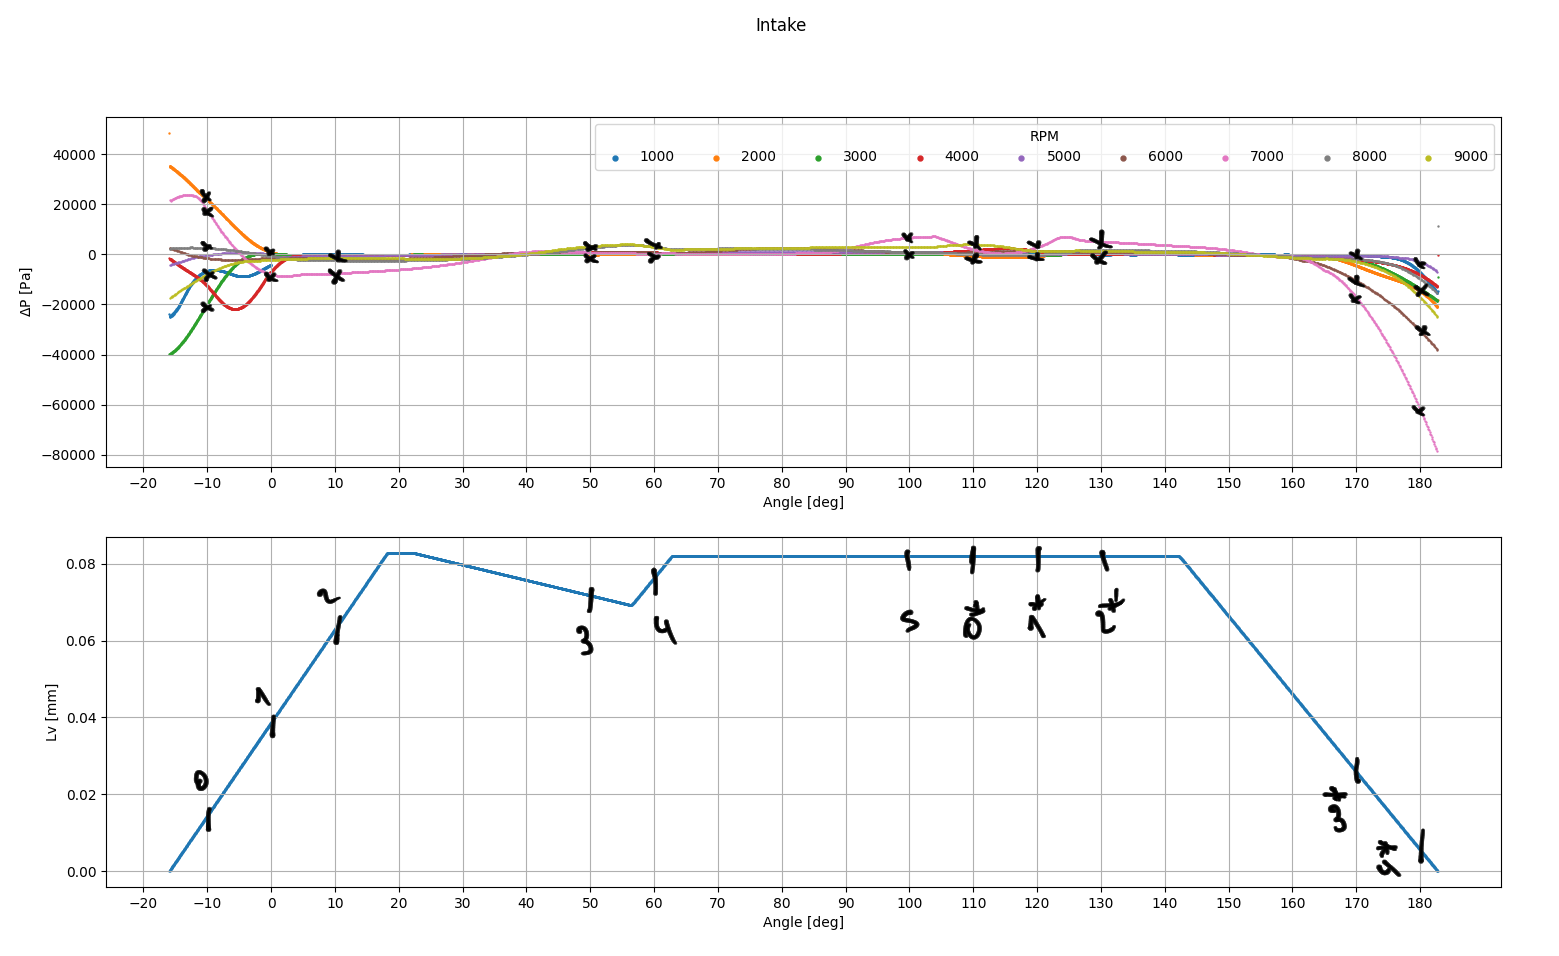
\includegraphics[width=1\textwidth]{flujometrias_admision.png}
    \caption{Flujometrías para el puerto de Admisión}\label{fig:flujometrias}
\end{figure}

\begin{table}
    \centering
    \begin{tabular}{rll} \toprule
        Caso & Ángulos  & Velocidades (rpm) \\ \midrule
        0    & -10, 110 & 1000, 2000, 3000, 7000, 8000 \\
        1    & 0, 120   & 2000, 7000 \\
        2    & 10, 130  & 2000, 7000 \\
        3    & 50, 170  & 3000, 7000, 9000 \\
        4    & 60, 180  & 3000, 5000, 6000, 7000 \\
        5    & 95       & 1000, 7000\\ \bottomrule
    \end{tabular}
    \caption{Flujometrías a realizar}\label{tab:casos}
\end{table}

Como se ve en la Figura~\ref{fig:flujometrias}, los puntos a evaluar son los
listados en la Tabla~\ref{tab:casos}.



\begin{figure}[h]
    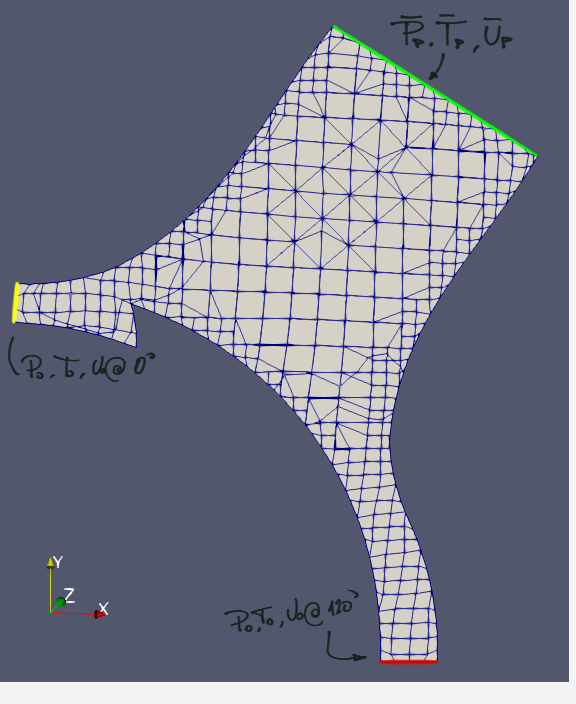
\includegraphics[width=0.8\textwidth]{caso_1-cc.png}
    \caption{Condiciones de borde}\label{fig:geom}
\end{figure}

Dentro del volumen de control, el campo de presiones se inicializa con el valor
medio de presiones de las cámaras y el campo de velocidades se hace
inicialmente (0,0,0).
%
El mapa de $C_D$ obetnido a partir de las flujoemtrías se lista en la
tabla~\ref{tab:mapaAdm} y~\ref{tab:mapaEsc} para los mapas de admisión y escape
respectivamente.


\begin{table}
  \parbox{.45\linewidth}{
  \centering
  \begin{tabular}{rccc}\toprule
    Item & $L_v[m]$ & $\Delta P[Pa]$ & $C_D$ \\ \midrule
    \lua{tex.print(mapaCd(myData.admision))}
    \bottomrule
    \end{tabular}
  \caption{Mapa $C_D$ del puerto de Admisión}\label{tab:mapaAdm}
  }
\hfill
\parbox{.45\linewidth}{
  \centering
  \begin{tabular}{rccc}\toprule
    Item & $L_v[m]$ & $\Delta P[Pa]$ & $C_D$ \\ \midrule
    \lua{tex.print(mapaCd(myData.escape))}
    \bottomrule
    \end{tabular}
  \caption{Mapa $C_D$ del puerto de Escape}\label{tab:mapaEsc}
}
\end{table}

\section{Segunda iteración y resultado final}
%
En la segunda iteración se utilizó el mapa de $C_D$ para la admisión y escape
como dato de entrada para ICESym, con esto se realizó una serie de corridas de
optimización con el algoritmo genético, de las cuales se seleccionaron los
mejores candidatos.
%
Se obtuvieron 3 candidatos principales, indicados como \emph{$run_34$},
\emph{$run_38$}, \emph{$run_51$}; cuyas curvas de rendimiento volumétrico y
fracción de gases residuales se indican en la figura \ref{fig:2iter_general}.
%
Para determinar cuál de todos es el más promoetedor, se compararon las curvas
de presión, torque y potencia, las cuales se muestran en las figuras
\ref{fig:2iter_presion}, \ref{fig:2iter_torque} y \ref{fig:2iter_potencia}
respectivamente.

